\chapter{Introduction}
\label{chap:intro}

\section{Background}
Computer networks have two classes of elements: the \textit{end hosts} that
generate packets and the \textit{routers}\footnote{We use the term router to
refer to both routers and switches in this disseration.} that forward packets
between the end hosts. Traditionally, computer networks have followed the
end-to-end principle~\cite{e2e}: the principle that most of the
application-specific logic or intelligence in a network should reside at the
end hosts, while the routers themselves should be fixed-function devices
dedicated to forwarding packets as efficiently as possible. This dichotomy can
be seen in any popular Internet application today. Whether it is video
conferencing, web browsing, or social networking, each application's
distinctive application logic resides in clients and servers, while the routers
themselves just take care of forwarding packets between these clients and
servers. The end-to-end principle has in part been responsible for the dramatic
success and heterogeneity of the Internet because it allows applications to
implement their own logic at end hosts without touching the networks' routers.

Yet, today's reality is very different from the pristine network architecture
presented by the end-to-end principle. It is increasingly clear that routers
need to implement far more than packet forwarding. A typical router box today
implements features that far exceeds just packet forwarding, such as access
control, measurement support, and tunneling, because these are important to
network operators. A single router box today covers functionality that spans a
few 1000 RFCs~\cite{lavanya_compiler}. Yet, there's little consensus among
operators and vendors as to what goes features go into a router, and the
routers themselves are fixed-function. Inevitably, there are operators whose
needs fall outside the laundry list of features implemented by routers. In such
cases, the operator is out of luck because there is no way to modify a
fixed-function router to add a new feature that makese sense to a particular
operator.

We are reaching a point where the rate of innovation in new router algorithms
is outstripping our ability to get these algorithms into production routers.
Figure~\ref{fig:router_algos} shows a timeline of prominent router algorithms
that have been developed since the 1980s. Of these, only a handful are
available in production routers because there is no easy way to implement a new
router algorithm on a production router.

%TODO: What are production routers? Define them.
\begin{figure}
\centering
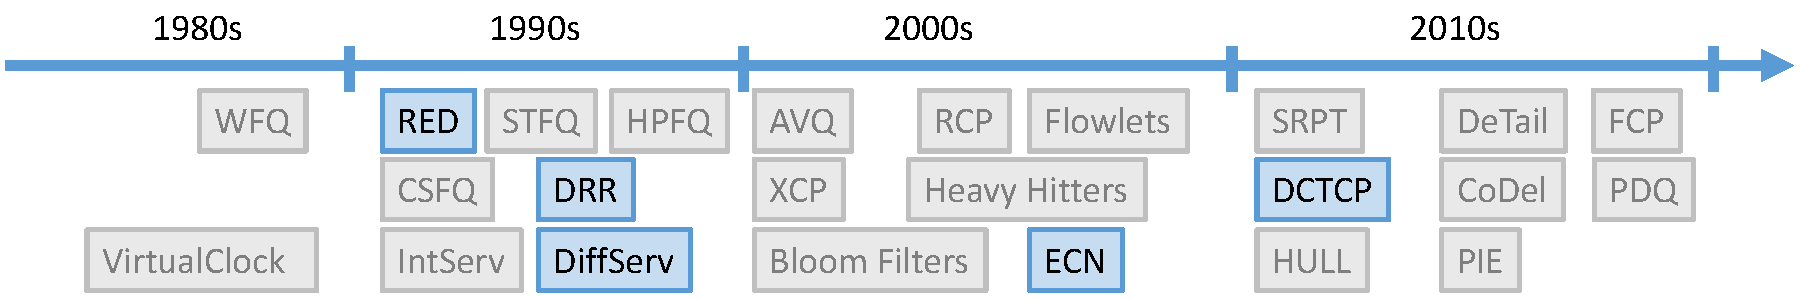
\includegraphics[width=\columnwidth]{router_alg_timeline.pdf}
\caption{Timeline of prominent router algorithms since the 1980s. Only the ones shaded in blue are available on production routers today.}
\label{fig:router_algos}
\end{figure}

As an operator who wants to implement some new functionality in a network, what
are the alternatives? One is to give up on changing routers altogether and make
all the required changes at the end hosts. But relying solely on end hosts
results in solutions that are cumbersome or suboptimal in many cases. As a
first example, imagine measuring the queuing latency at a particular hop in the
network by collecting end-to-end ping measurements between a variety of vantage
points and then fusing these measurements together to estimate per-hop queueing
latency. Not only is this indirect, it is also inaccurate relatively to just
instrumenting the router to measure it's own queueing latency. As a second
example, consider the problem of congestion control, which divides up a
network's capacity in some fair manner among competing users. There are many
in-network solutions to congestion control are superior in performance to the
end-host-only approaches to congestion control that are deployed today. Yet,
there is no way to deploy these in-network solutions today.

Another alternative for operators is to use a \textit{software router}: a
catch-all term for a router built on top of some \textit{programmable}
substrate, such as a general-purpose CPU, a network processor (a CPU with some
instructions tailored to packet processing), a GPU, or an FPGA. There are many
examples of such software routers~\cite{click, routebricks, netfpga,
packetshader, ixp4xx, ixp2800}. Figure~\ref{fig:router_evolution} tracks the aggregate
capacity of software routers over time and compares them against the fastest
routers known at a given point in time. The figure shows two trends. First, up
until the mid 90s, software routers were in fact the fastest routers; the early
routers were just minicomputers with special forwarding software. However,
since the mid 90s, growing demands for higher link speeds, fueled by the
Internet's explosive growth, have meant that the fastest routers tend to be
built out of dedicated hardware, specialized to packet forwarding. Further, the
performance of these routers is between 10 and 100 $\times$ better than
software routers. However, because these routers are built of specialized
hardware, they tend to be fixed-function and can not be programmed in the field
unlike software routers. While recent work in software-defined
networking~\cite{openflow} and programmable data planes~\cite{rmt, flexpipe,
xpliant, tofino} has made such fast routers flexible to some degree, these
solutions are still not sufficient to express the algorithms shown in
Figure~\ref{fig:router_algos}.

\begin{figure}
\centering
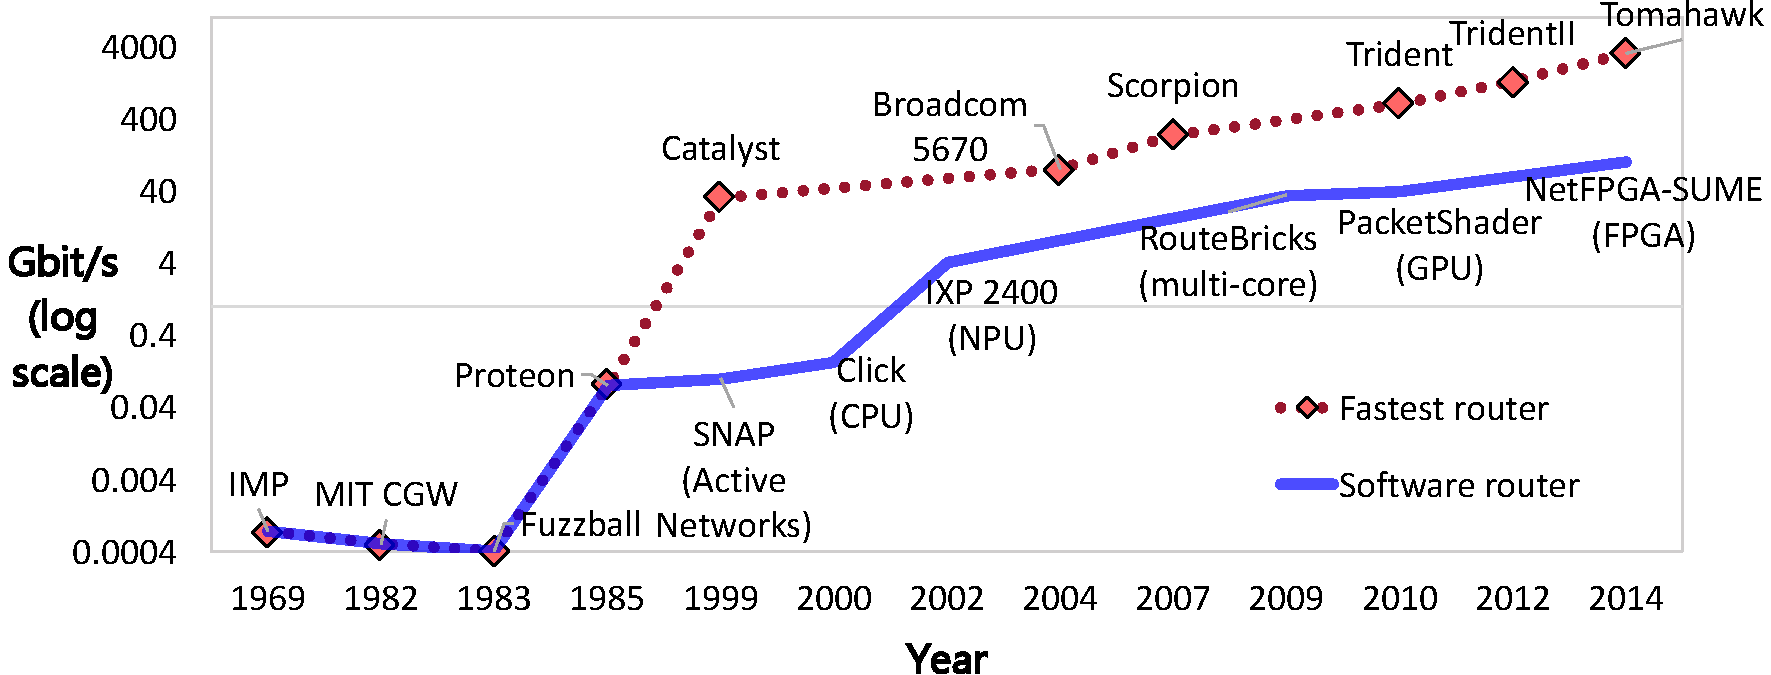
\includegraphics[width=\columnwidth]{router_evolution.pdf}
\caption{Aggregate capacity of routers since the first router on the ARPANET in
1969~\cite{imp}. Until the mid 90s, software routers were sufficient; since
then, however, the fastest routers have been built out of dedicated hardware.}
\label{fig:router_evolution}
\end{figure}

\section{Primary Contributions}

This dissertation considers the problem of building routers that are both fast
(\ie approaching the speed of the fastest fixed-function routers today), while
also being programmable. In particular, my thesis is that it is possible to
design router hardware that is both fast and programmable, as long as we
restrict ourselves to specific classes of router functionality. It is this
specificity that allows us to resolve this tension between programmability and
performance; indeed, our designs provide a much more restricted form of
programmability than a Turing-complete processor. The challenge here is to pick
classes of router functionality that are actually practically useful to network
operators, broad enough to cover a range of current and future use cases within
that class, yet narrow enough to permit a high-speed hardware implementation.

This dissertation will describe high-speed programmable hardware designs and
their corresponding programming models in software that target three such
classes of router functionality: stateful data-plane algorithms, packet
scheduling, and scalable network measurement.

\subsection{Stateful data-plane algorithms}
Domino (Chapter~\ref{chap:domino}) is a system to program \textit{data-plane
algorithms} on high-speed router hardware. Data-plane algorithms operate on a
sequeunce of packets, doing a bounded amount of work per packet and
manipulating a bounded amount of router state in the process.  They include
algorithms for managing the router's buffer, load balancing, and in-network
congestion control.

High-speed data-plane programming poses two challenges: (1) what hardware instructions are required to support programmable state modification at the router’s line rate and (2) what is the right programming model? In addressing each challenge, Domino makes two new contributions.

First, \textit{Atoms} capture a router’s instruction set. They specify atomic
units of packet processing provided by the router hardware, e.g., an atomic
counter or an atomic test-and-set. Atoms are atomic in that all state updated
by an atom is visible to the next packet arriving at the atom in the next clock
cycle.

Second, \textit{Packet Transactions} provide a programming model. A packet
transaction is an atomic and isolated block of code capturing an algorithm’s
logic. It provides the semantics that any visible state is equivalent to a
serial execution of packet transactions in the order of packet arrival—akin to
an infinitely fast single-threaded router. Packet transactions are expressive
and capture many important data-plane algorithms. Further, their serial
semantics shield programmers from the hardware’s parallelism, instead enlisting
a compiler to transform a serial packet transaction to a parallel atom
pipeline.

Together, atoms and packet transactions allow us to program several algorithms
from Figure~\ref{fig:router_algos} (\eg the Adaptive Virtual Queue~\cite{avq}
active queue management algorithm, the CONGA~\cite{conga} load balancing
algorithm, bloom filters for measurement, and count-min sketches for detecting
heavy hitters) on speeds approaching high-speed routers for the first time. P4
[2], a packet-processing language that is emerging as an industry standard for
programming router chips, has adopted packet transactions.  P4 programmers can
now use an @atomic annotation around a block of statements to specify that the
block must execute atomically.

\subsection{Packet scheduling}

Packet scheduling is an important determinant of network performance. The
choice of scheduling algorithm is tied to a network’s overarching goals. For
instance, an algorithm that divides link capacity fairly is ideal in a
multi-tenant setting, while the shortest remaining processing time algorithm is
ideal for a single tenant who desires low flow completion time. Today’s routers
provide a fixed set of scheduling algorithms and do not allow an operator to
program scheduling to suit their needs.

Routers lack programmable scheduling because there is no single abstraction to
express many scheduling algorithms. Push In First Out Queues (PIFOs) provide
such an abstraction. They exploit the fact that in many practical schedulers,
the relative order of packets that are already buffered does not change in
response to new packet arrivals. Put differently, when a packet arrives, it can
be pushed into the right location based on a packet priority (push in), but
packets can always be dequeued from the head (first out). The PIFO abstraction
is simple: a priority queue of packets with a small program to assign each
packet its priority. Yet, by flexibly programming a packet’s priority
assignment, a network operator can use the PIFO abstraction to program a
variety of previously proposed scheduling algorithms. So far, these algorithms
could only be run in simulation or on slower speed software routers.
%TODO: Could improve flow here.
A single PIFO expresses many schedulers, e.g., token bucket shaping, weighted
fair queueing, and strict priority scheduling. Further, PIFOs can be combined
to express hierarchical schedulers. Finally, PIFOs are feasible in hardware: a
hardware design for a programmable 5-level hierarchical scheduler costs less
than 4\% additional chip area.

\subsection{Scalable network measurement}

\textit{Performance Queries} provide a query language and supporting router
hardware for network performance measurement queries. As examples, an operator
could ask for flows with a high degree of packet reordering or a moving average
of packet latencies for each flow. Our query language allows order-dependent
aggregation (e.g., an exponentially weighted moving average over packet
latencies), while traditional query languages (\eg SQL) only supports
order-independent aggregates like counts and averages. The router hardware to
support these queries is a programmable key-value store in the router’s ASIC.
The keys represent flows, while the values store and programmatically update
per-flow state (\eg counters or a moving average filter) on every packet.

At the heart of our this key-value store is a technique to scalably aggregate
information across packets belonging to a flow, while scaling to a large number
of flows. We formally characterize the set of state update functions that allow
us to scalably implement aggregations across a large number of flows.
% TODO: The paragraph above needs work

\section{Towards a world of programmable networks}

The results in this dissertation point towards a world of programmable
networks, where routers within a network are \textit{told} what to do by their
operators, without the router vendors telling their operators what they can
support. In such a setting, operators could customize networks as they see fit.
They could program additional features that give them performance benefits.
More interestingly, they could remove needless features from their router,
allowing them to simplify their routers' feature sets, which in turn would ease
troubleshooting when things go wrong.

Besides the benefits to network operators, a programmable router chip set has
benefits for router vendors as well. Router vendors can now add new features in
firmware and sell different versions of the firmware to different market
segments. Further, when bugs arise, it is much easier to fix these bugs in
firmware, as opposed to redoing the hardware design for the router (which could
easily take a year). It also allows them to respond to new requests from
network operators in a period of days as opposed to years.

Whether the specific classes of programmability this dissertation provides will
be sufficient and future proof remains to be seen, but we are encouraged by the
fact that the hardware designs proposed here support a wide range of existing
use cases and several new use cases that we had not anticipated initially. We
hope these results provide guidance to router chip manufacturers when designing
hardware for programmable routers.
